\section{Objective}
\label{sec:4-1}

Data Understanding and Data Preparation (Chapter~\ref{ch:data-preparation}) form one narrative: understand the data, extract insights about transactions and customers, and turn them into the strategy for building the modeling dataset -- its population, label and features. The business question behind this chapter is which customers to prioritize for retention or promotion activities, so that expected future margin grows without discounting more than necessary.

This chapter covers the first half of the narrative: an overview of the data (Section~\ref{sec:4-2}), sales and seasonality (Section~\ref{sec:4-3}), RFM features (Section~\ref{sec:4-4}), how often customers come back (Section~\ref{sec:4-5}), RFM customer segments with their retention and weekly dynamics (Section~\ref{sec:4-6}) and how revenue is concentrated across customers (Section~\ref{sec:4-7}). It ends with the design decisions (Section~\ref{sec:4-8}) that Chapter~\ref{ch:data-preparation} implements.

\section{Dataset Overview}
\label{sec:4-2}

The raw dataset (before any cleaning) contains:

\begin{center}
\begin{tabular}{@{}p{5cm}p{8.5cm}@{}}
    \toprule
    Metric & Value \\
    \midrule
    Transactions (rows) & 1,067,371 \\
    Invoices & 53,628 \\
    Customers & 5,942 \\
    Products & 5,305 \\
    Countries & 43 \\
    Total quantity & 10,608,492 units \\
    Total revenue (GBP) & 19,287,250.57 \\
    Date range & 2009-12-01 -- 2011-12-09 ($\approx$ 2 years) \\
    \bottomrule
\end{tabular}
\end{center}

The dataset is overwhelmingly UK-based: the \textbf{United Kingdom} accounts for 981,330 rows (91.9\%); the next largest markets are EIRE (17,866), Germany (17,624), France (14,330) and the Netherlands (5,140), each far behind the UK.

After applying the valid-purchase definition (Section~\ref{sec:5-2}), \textbf{776,577 rows (72.8\%) remain, representing 36,594 purchase occasions (invoices) of 5,852 customers} between 1 December 2009 and 9 December 2011. The RFM analysis of this chapter (Sections~\ref{sec:4-4}, \ref{sec:4-6} and~\ref{sec:4-7}) starts from the cleaned transaction file, which keeps returns as negative-revenue rows: 794,165 rows of 5,875 customers with a Customer ID, of whom \textbf{5,852 have at least one sale}. Returns are netted against sales when monetary value is computed.

\section{Monthly Sales and Seasonality}
\label{sec:4-3}

\begin{center}
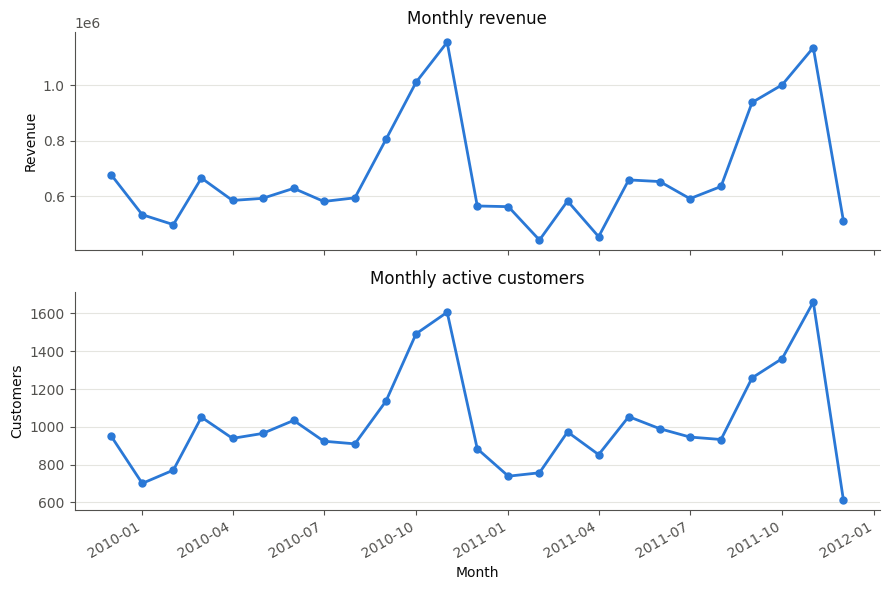
\includegraphics[width=0.85\textwidth]{figures/ch6_monthly_revenue_customers.png}
\end{center}

A typical full month has about \textbf{1,040 purchasing customers} (median 965) and \textbf{revenue of about GBP 690K} (median GBP 595K), ranging from GBP 442K (Feb 2011) to GBP 1.16M (Nov 2010). Both series are clearly \textbf{seasonal}: a steady climb from late summer to a peak in \textbf{October--November} (Nov 2010: GBP 1.16M; Nov 2011: GBP 1.14M; Oct 2010 and Oct 2011: GBP 1.0M each), driven by pre-Christmas ordering, followed by a sharp fall in December (Dec 2010: GBP 565K, 884 customers) through February. The first month (Dec 2009) and the last month (Dec 2011, only 9 days of data) are partial periods.

Two consequences carry into Chapter~\ref{ch:data-preparation}. Only about 1,040 of the 5,852 customers buy in a given month, so most customers purchase infrequently and churn must be judged over a window much longer than a month. And because behavior shifts with the season, the data must be split chronologically and results read per scoring week.

\section{RFM Features}
\label{sec:4-4}

Each customer is described by recency, frequency and monetary value (RFM), computed over the \textbf{whole history} and measured against the day after the last transaction in the data (10 December 2011). This view is descriptive: model features in Chapter~\ref{ch:data-preparation} use only history up to each snapshot date.

\begin{center}
\small
\begin{tabular}{@{}p{3.4cm}p{6.2cm}p{4.9cm}@{}}
    \toprule
    Feature & Definition & Why \\
    \midrule
    \texttt{recency\_days} (R) & Days from the last \emph{purchase} to the reference date & Returns are not purchase activity \\
    \texttt{frequency} (F) & Distinct sales invoices & Counts purchase occasions \\
    \texttt{monetary} (M) & Sales minus returned value, floored at 0 & Returns erode real customer value \\
    \texttt{avg\_order\_value} & Gross sales $/$ F & Separates large-basket from small-basket customers \\
    \texttt{return\_rate} & Returned value $/$ gross sales & Returns erode margin \\
    \texttt{tenure\_days} & Days since the customer first appeared & Long-standing vs.\ new customers \\
    \texttt{avg\_gap\_days} & Mean days between consecutive purchase days & The customer's own rhythm \\
    \texttt{recency\_gap\_ratio} & R $/$ \texttt{avg\_gap\_days} & $>1$: silent for longer than usual \\
    \texttt{frequency\_90d}, \texttt{monetary\_90d} & F and M over the last 90 days & Recent activity \\
    \bottomrule
\end{tabular}
\end{center}

The rhythm and 90-day columns are not used to define segments; they only describe customers in more detail. Distribution of the 5,852 customers with at least one sale:

\begin{center}
\small
\begin{tabular}{@{}lrrrrr@{}}
    \toprule
    Feature & Mean & Median & P90 & P99 & Max \\
    \midrule
    Recency (days) & 199.7 & 95 & 530 & 726 & 738 \\
    Frequency (invoices) & 6.25 & 3 & 13 & 46 & 373 \\
    Monetary (GBP) & 2,795.90 & 840.25 & 5,224.45 & 26,490.31 & 578,408.64 \\
    Average order value (GBP) & 384.40 & 277.87 & 624.03 & 1,907.11 & 84,236.25 \\
    Return rate & 0.02 & 0.00 & 0.05 & 0.39 & 2.86 \\
    \bottomrule
\end{tabular}
\end{center}

\begin{center}
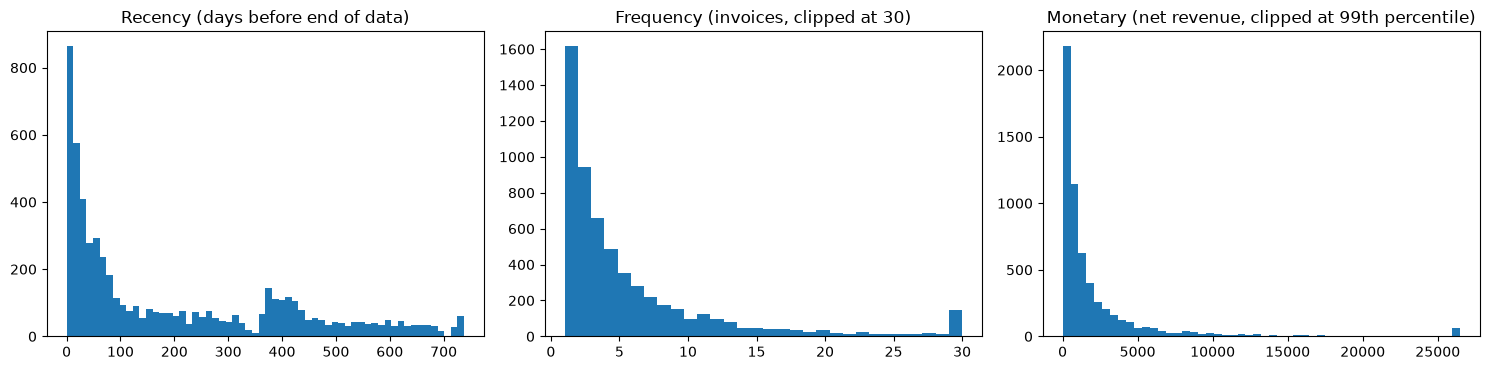
\includegraphics[width=\textwidth]{figures/ch6_rfm_distributions.png}
\end{center}

All three RFM variables are strongly right-skewed: the median customer bought three times and spent GBP 840, while the mean monetary value (GBP 2,796) is more than three times the median. Recency is spread over the whole two-year range, with a large mass of customers who have been silent for more than a year. Two cautions apply. First, F and M are cumulative, so customers present since December 2009 have had more time to accumulate them than newer customers. Second, F counts invoices, not visits: for 20.8\% of customers F differs from the number of distinct purchase days because they issued several invoices on the same day (typical of wholesale accounts, which split orders by warehouse or product type), so a customer with F $=$ 4 has not necessarily come back four times.

\section{Repurchase Interval and the 90-Day Horizon}
\label{sec:4-5}

Retail is a \textbf{non-contractual} setting: customers never cancel, so churn has to be inferred from a period without purchases. The gap between consecutive purchase occasions of the same customer tells how long that period should be. Note that the shares below are per \textbf{repurchase} (one gap per repeat occasion, 30,742 in total), not per customer: frequent buyers contribute more gaps, and one-time customers contribute none.

\begin{center}
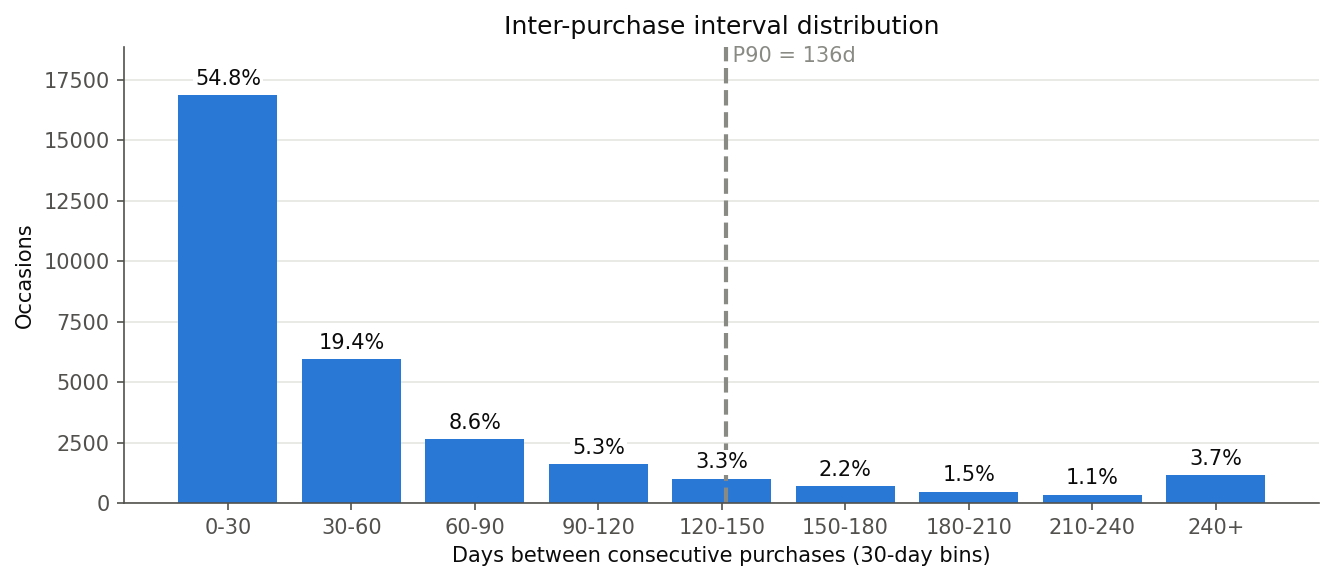
\includegraphics[width=0.85\textwidth]{figures/ch6_inter_purchase_interval.png}
\end{center}

\begin{center}
\begin{tabular}{@{}p{2.3cm}p{2.3cm}p{2.3cm}p{2.3cm}p{2.3cm}@{}}
    \toprule
    Mean & Std & Median & P90 & P99 \\
    \midrule
    52.1 d & 75.9 d & 25.0 d & 136.0 d & 368.9 d \\
    \bottomrule
\end{tabular}
\end{center}

Gaps are highly right-skewed (mean 52.1 days vs.\ median 25.0 days). \textbf{54.8\% of repurchases happen within 30 days} of the previous purchase -- the largest single group, but not yet representative of repurchasing as a whole. Extending the window to \textbf{90 days covers 82.8\% of repurchases}; beyond 150 days each 30-day bin holds under 2.5\% of gaps, and the open-ended 240+ bin collects the remaining 3.7\%.

\textbf{Choosing the horizon $H$.} The prediction horizon trades off three criteria:

\begin{center}
\begin{tabular}{@{}p{1.6cm}p{5cm}p{4.6cm}@{}}
    \toprule
    $H$ (days) & Repurchases within $H$ & Training weeks after the embargoed split \\
    \midrule
    60 & 74.2\% & 37 \\
    \textbf{90} & \textbf{82.8\%} & \textbf{24} \\
    120 & 88.1\% & 10 \\
    \bottomrule
\end{tabular}
\end{center}

A shorter horizon labels as churned many customers who would in fact come back (noisier labels); a longer one detects churn later -- at odds with the goal of early identification (Section~\ref{sec:1-2}) -- and, on a two-year window, leaves far fewer labelable weeks for training once two $H$-day embargoes are subtracted (computed in Section~\ref{sec:5-6}). \textbf{$H = 90$ days} covers most repurchases while keeping 24 training weeks; moving to 120 days would add only 5 points of coverage at the cost of more than half the training weeks. The 90-day mark also matches the ``active'' boundary used by the RFM segments of Section~\ref{sec:4-6}.

The same distribution sets the \textbf{activity threshold} $R_{\max} = $ P90 $=$ 136 days: a customer whose last purchase is older than this is treated as already lapsed and is not scored. $H$ answers \emph{how long without a purchase counts as churn}; $R_{\max}$ answers \emph{who is still worth predicting for}.

\textbf{Per repurchase vs.\ per customer.} The 82.8\% above is a share of repurchases, dominated by frequent buyers. Per customer, the picture is less favorable: 1,618 customers (27.7\% of the base) bought only once and have no repurchase at all, and among repeat customers only \textbf{59.8\%} have an average gap under 90 days (17.8\% under 30 days, 41.9\% at 30--90 days) while 40.2\% buy more slowly. This explains why the churn rate at $H = 90$ is close to one half (Section~\ref{sec:5-4}) even though most repurchases happen within 90 days.

\section{RFM Customer Segments}
\label{sec:4-6}

\subsection{Segmentation rules}

Customers are assigned to one of eight segments by rules applied \textbf{in order}; a customer falls into the first rule that holds, so segments are mutually exclusive and cover every customer. The thresholds are business conventions with the following anchors: R at 90, 180 and 365 days (customers become ``cool'' after 90 days without a purchase, ``lapsed'' after 180 and almost gone after a year); F at 1 / 2--3 / 4+ invoices; and ``high value'' as monetary value in the top 10\% of customers (GBP 5,224.45, Section~\ref{sec:4-7}).

\begin{center}
\small
\begin{tabular}{@{}clp{4.6cm}p{5.4cm}@{}}
    \toprule
    \# & Segment & Rule & Meaning \\
    \midrule
    1 & Champions & M $\ge$ top 10\% and R $\le$ 90 & Highest value, still active \\
    2 & VIP at risk & M $\ge$ top 10\% and R $>$ 90 & Once high value, silent for a while \\
    3 & Loyal & R $\le$ 90 and F $\ge$ 4 & Buys regularly, medium value \\
    4 & Developing & R $\le$ 90 and F = 2--3 & Has repurchased, not yet a habit \\
    5 & One-time recent & R $\le$ 90 and F = 1 & Recently bought for the first time \\
    6 & Cooling & 90 $<$ R $\le$ 180 & Going cold \\
    7 & Lapsed & 180 $<$ R $\le$ 365 & Away for long, can still be won back \\
    8 & Dormant & R $>$ 365 & Almost certainly gone \\
    \bottomrule
\end{tabular}
\end{center}

These segments are a descriptive, business-facing view of the whole history. They are \emph{not} the six train-fitted RFM segments that Section~\ref{sec:5-5} builds from quintile scores for the modeling dataset.

\subsection{Segment profile}

\begin{center}
\small
\setlength{\tabcolsep}{4pt}
\begin{tabular}{@{}lrrrrrr@{}}
    \toprule
    Segment & Cust. & \% cust. & Med.\ R (d) & Med.\ F & Med.\ M (GBP) & \% revenue \\
    \midrule
    Champions & 515 & 8.8\% & 11 & 20 & 8,945.53 & 58\% \\
    VIP at risk & 71 & 1.2\% & 184 & 13 & 8,550.92 & 5\% \\
    Loyal & 1,345 & 23.0\% & 24 & 7 & 2,070.71 & 19\% \\
    Developing & 658 & 11.2\% & 29 & 2 & 663.66 & 3\% \\
    One-time recent & 367 & 6.3\% & 44 & 1 & 256.32 & 1\% \\
    Cooling & 555 & 9.5\% & 131 & 3 & 868.77 & 4\% \\
    Lapsed & 777 & 13.3\% & 260 & 2 & 566.13 & 4\% \\
    Dormant & 1,564 & 26.7\% & 468 & 1 & 338.56 & 5\% \\
    \bottomrule
\end{tabular}
\end{center}

\begin{center}
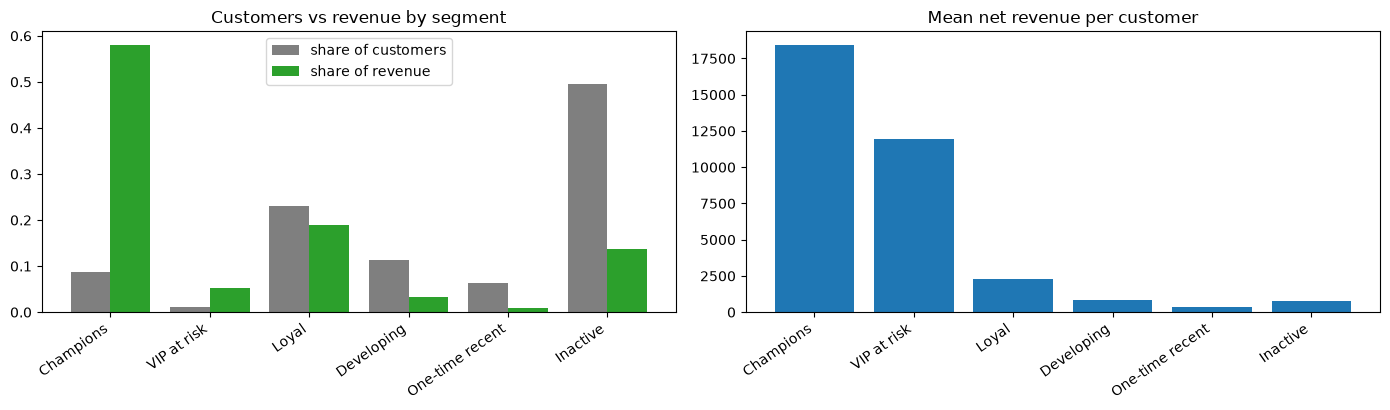
\includegraphics[width=0.95\textwidth]{figures/ch6_rfm_segment_share.png}
\end{center}

(In the chart, Cooling, Lapsed and Dormant are merged into one \emph{Inactive} group: 2,896 customers, 49.5\% of the base, about 13\% of revenue.)

Revenue is carried by very few customers. \textbf{Champions} are 8.8\% of customers but about \textbf{58\%} of revenue, and together with Loyal customers they hold about 77\%. At the other end, Dormant customers are over a quarter of the base but only about 5\% of revenue. \textbf{VIP at risk} is the smallest segment (71 customers) yet holds about 5\% of revenue with a median monetary value of GBP 8,551 -- almost the same as Champions -- and has been silent for a median of 184 days, which makes it the clearest candidate for retention effort.

\subsection{Cohort retention}

Customers are grouped by the month of their first purchase. Each cell of the retention matrix is the share of a cohort that bought in the $k$-th month after its first month. Weighted over all cohorts from January 2010 (the December 2009 cohort is excluded because it includes customers who had already bought before the data starts), the share of customers who buy in a given month is:

\begin{center}
\small
\begin{tabular}{@{}lrrrrrrrrrrrr@{}}
    \toprule
    Month $k$ & 1 & 2 & 3 & 4 & 5 & 6 & 7 & 8 & 9 & 10 & 11 & 12 \\
    \midrule
    Retention & 21\% & 21\% & 21\% & 19\% & 19\% & 18\% & 18\% & 16\% & 15\% & 13\% & 14\% & 18\% \\
    \bottomrule
\end{tabular}
\end{center}

\begin{center}
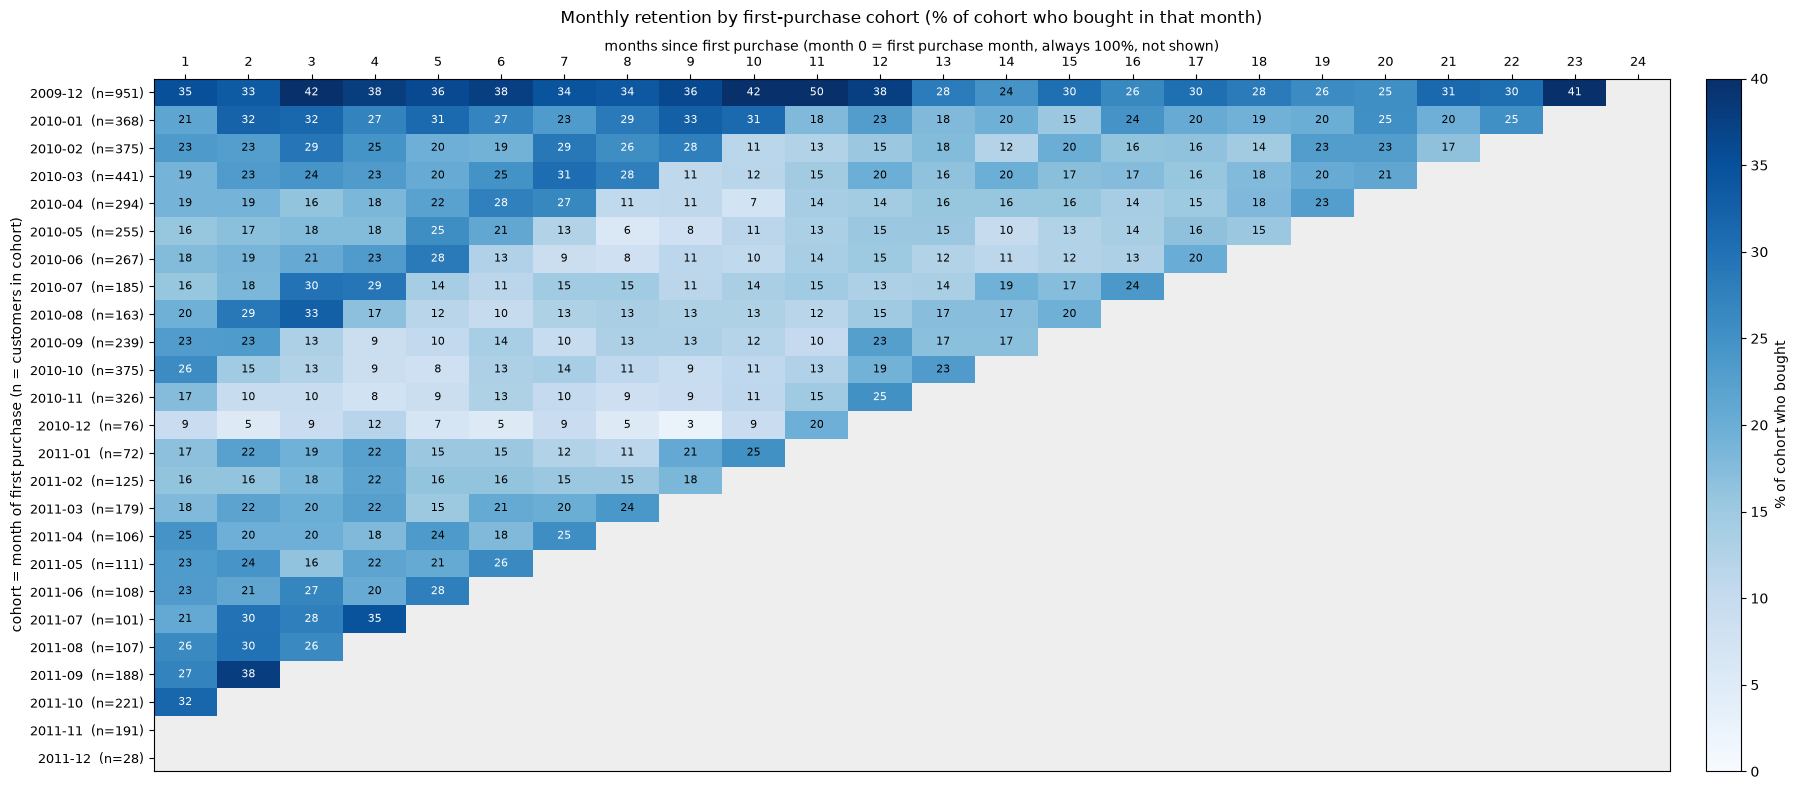
\includegraphics[width=\textwidth]{figures/ch6_cohort_retention_heatmap.png}
\end{center}

\begin{itemize}
    \item \textbf{New customers return most in the first two or three months} (about 21\% buy in each of months 1--3), then retention drifts down to 13--16\%; the first months after a first purchase are the main window to win a second purchase.
    \item \textbf{Seasonality shows up as dark diagonals.} For example, the August 2010 cohort reaches 33\% in month 3 (November 2010) and the September 2011 cohort reaches 38\% in month 2 (November 2011). Such cells are dark because they fall in the peak season, not because the cohort is better; cohorts should be compared at the same age.
    \item \textbf{The December 2010 cohort retains worst} (3--12\% in most months, 76 customers): customers acquired just after the peak season rarely come back.
    \item The 2011 cohorts look steadier than mid-2010 ones, but they have been observed for at most ten months, and early months are always higher than late ones, so no conclusion is drawn.
\end{itemize}

\begin{center}
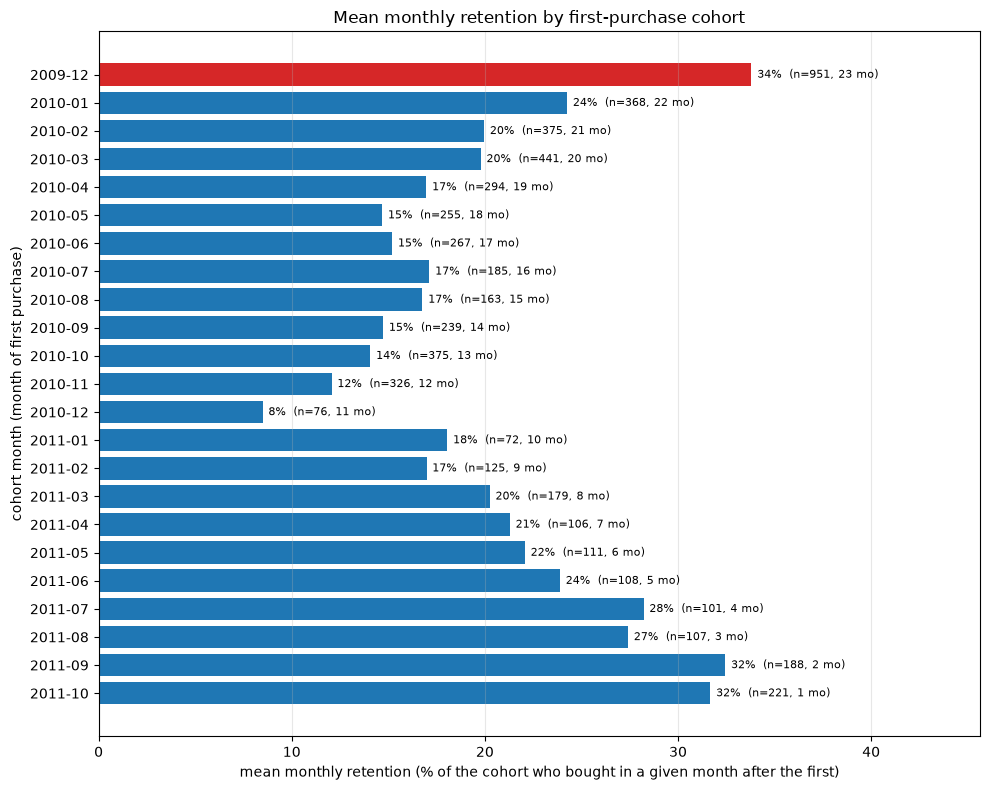
\includegraphics[width=0.8\textwidth]{figures/ch6_cohort_retention_bar.png}
\end{center}

The bar chart condenses each cohort into one number, the mean monthly retention over its fully observed months. It is a quick comparison only: recent cohorts are averaged over one to three ``easy'' months right after the first purchase (and two of them fall in the peak season), so their bars look tall; compare cohorts of similar observed length, or use the heatmap column by column.

\subsection{Weekly segment dynamics}

The same rules are applied at every Monday snapshot (105 snapshots, from 7 December 2009 to 5 December 2011) using the history up to that date; the ``high value'' threshold is recomputed every week as the top 10\% of cumulative monetary value, since cumulative M only grows (it rises from about GBP 1,000 to about GBP 5,200). The number of customers per segment at selected snapshots:

\begin{center}
\small
\begin{tabular}{@{}lrrrrrrrr@{}}
    \toprule
    Snapshot & Champ. & VIP at risk & Loyal & Devel. & One-time & Cooling & Lapsed & Dormant \\
    \midrule
    2009-12-07 & 43 & 0 & 2 & 31 & 349 & 0 & 0 & 0 \\
    2010-02-15 & 152 & 0 & 60 & 400 & 905 & 0 & 0 & 0 \\
    2010-07-05 & 285 & 13 & 433 & 709 & 629 & 699 & 211 & 0 \\
    2010-12-06 & 396 & 31 & 978 & 858 & 652 & 579 & 747 & 28 \\
    2011-06-20 & 431 & 67 & 895 & 427 & 260 & 598 & 1,650 & 652 \\
    2011-12-05 & 513 & 71 & 1,328 & 649 & 377 & 556 & 791 & 1,550 \\
    \bottomrule
\end{tabular}
\end{center}

\begin{center}
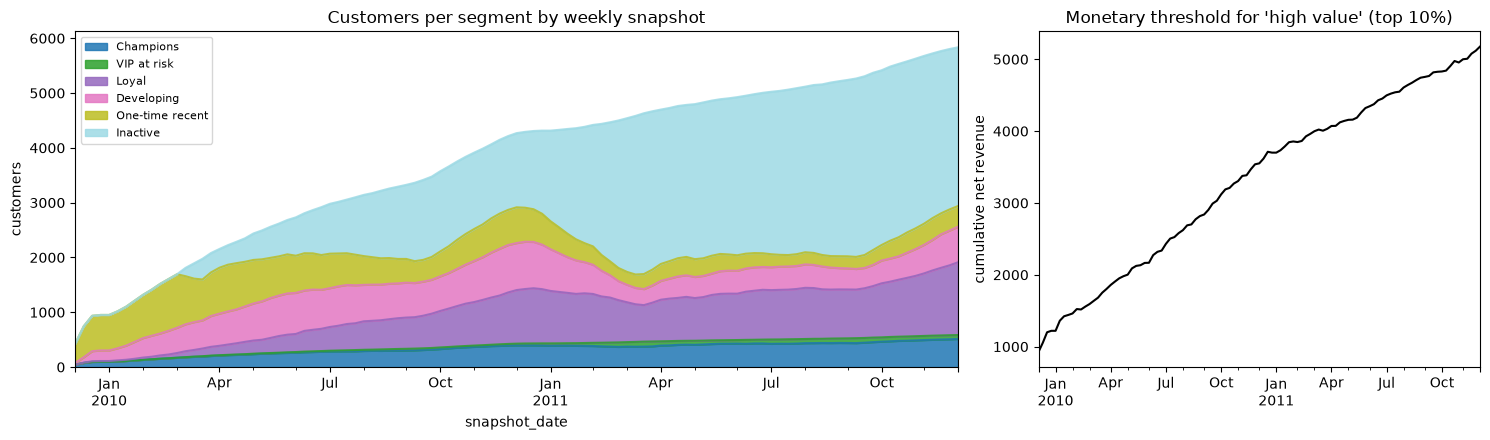
\includegraphics[width=\textwidth]{figures/ch6_weekly_segments.png}
\end{center}

\begin{itemize}
    \item \textbf{The base only grows.} A customer who has ever bought stays in the table, so total height (4,269 customers on 2010-12-06, 5,835 on 2011-12-05) counts customers ever seen, not customers currently active. The growth of Lapsed and Dormant (Dormant: 28, then 652, then 1,550) is cumulative history, not a deterioration in behavior.
    \item \textbf{Post-peak cooling.} Cooling jumps after the Q4 peak (579 on 2010-12-06 to a peak of 1,679 on 2011-03-14) and shrinks again (646 on 2011-06-06) as these customers cross 180 and 365 days and move into Lapsed and Dormant. At the same time One-time recent (652 down to 244) and Developing (858 down to 299) shrink: customers won during the peak season largely do not return within 90 days.
    \item \textbf{Champions and Loyal grow steadily} (Champions 396 to 513; Loyal 978 to 1,328 between 2010-12-06 and 2011-12-05) and are the least affected by the season.
    \item \textbf{VIP at risk is small but seasonal}: 31 on 2010-12-06, a peak of 88 on 2011-03-14, then 71 -- high-value customers who go quiet after the peak season, some of whom return.
\end{itemize}

Week-to-week transitions between segments (customers present in both weeks; Cooling, Lapsed and Dormant merged into \emph{Inactive}) show how likely the important events are in a single week:

\begin{center}
\small
\begin{tabular}{@{}p{5.6cm}rrr@{}}
    \toprule
    Event & Customer-weeks in source segment & Transitions & Weekly rate \\
    \midrule
    Loyal $\to$ Champions & 66,034 & 565 & 0.86\% \\
    Champions $\to$ VIP at risk & 34,602 & 431 & 1.25\% \\
    Champions $\to$ Inactive & 34,602 & 7 & 0.02\% \\
    VIP at risk $\to$ Champions & 4,330 & 291 & 6.72\% \\
    VIP at risk $\to$ Inactive & 4,330 & 69 & 1.59\% \\
    \bottomrule
\end{tabular}
\end{center}

Champions almost never drop straight to Inactive (0.02\% per week); they first pass through VIP at risk (1.25\% per week), which is therefore the early-warning stage. From VIP at risk, a customer is about four times more likely to return to Champions (6.72\% per week) than to fall into Inactive (1.59\%), so a customer in this state is still recoverable -- the window in which a retention action is most useful.

\section{Value Concentration}
\label{sec:4-7}

Revenue is concentrated in a small number of large, often wholesale, customers. Measured per customer as net revenue over the full history:

\begin{center}
\begin{tabular}{@{}p{3.6cm}p{4.2cm}p{3.2cm}@{}}
    \toprule
    Customers (by revenue) & Revenue threshold (GBP) & Share of revenue \\
    \midrule
    Top 1\% & 26,679.24 & 31\% \\
    Top 5\% & 8,945.53 & 51\% \\
    Top 10\% & 5,250.78 & 63\% \\
    Top 20\% & 2,835.36 & 77\% \\
    Top 30\% & 1,743.15 & 85\% \\
    Top 50\% & 840.25 & 93\% \\
    \bottomrule
\end{tabular}
\end{center}

\begin{center}
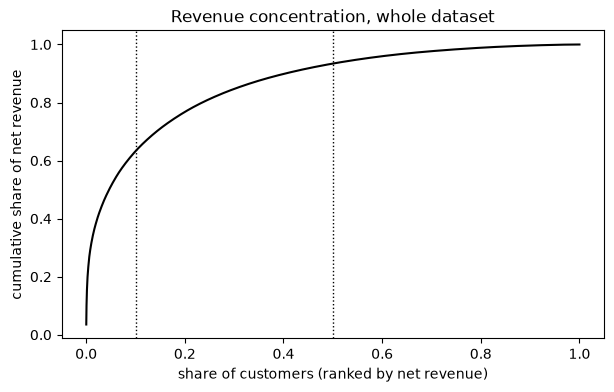
\includegraphics[width=0.6\textwidth]{figures/ch6_rfm_pareto.png}
\end{center}

The top 10\% of customers (monetary value of at least GBP 5,224.45, the ``high value'' threshold of Section~\ref{sec:4-6}) hold 63\% of revenue and the bottom half only 7\%. The average order value reaches GBP 1,907 at the 99th percentile and GBP 84,236 at the maximum, so any value-weighted measure -- revenue at risk, expected margin -- would be dominated by a handful of wholesale-sized accounts. This motivates capping the customer value proxy V at its 99th percentile, fitted on the training period (Section~\ref{sec:5-5}), and reporting wholesale-sized customers separately in the error analysis (Section~\ref{sec:7-12}).

\section{Key Findings and Design Decisions}
\label{sec:4-8}

\begin{center}
\small
\begin{tabular}{@{}p{7.2cm}p{7cm}@{}}
    \toprule
    Finding & Design decision (Chapter~\ref{ch:data-preparation}) \\
    \midrule
    776,577 valid rows (72.8\%) = 36,594 invoices of 5,852 customers, Dec 2009 -- Dec 2011 & Customer histories built from valid purchase occasions only (Sections~\ref{sec:5-2}--\ref{sec:5-3}) \\
    About 1,040 customers and GBP 690K revenue per month; peak in Oct--Nov, sharp drop in Dec; Cooling jumps after Q4 and the December 2010 cohort retains worst & Chronological split with embargo; results read per scoring week (Section~\ref{sec:5-6}) \\
    Only about 1,040 of 5,852 customers buy in a given month & Weekly snapshots of all active customers, judged over a multi-month window (Section~\ref{sec:5-3}) \\
    54.8\% of repurchases within 30 days, 82.8\% within 90 days; P90 gap $=$ 136 days & Label horizon $H = 90$ days (Section~\ref{sec:5-4}); activity threshold $R_{\max} = 136$ days (Section~\ref{sec:5-3}) \\
    Champions (8.8\% of customers) and Loyal customers hold about 77\% of revenue; Dormant customers are 26.7\% of customers but about 5\% of revenue & Scoring population limited to customers still active ($R \le R_{\max}$), where retention effort can still change the outcome (Section~\ref{sec:5-3}) \\
    New customers return mostly in the first two or three months; one-time customers are 27.7\% of the base & One-time customers kept in the population but reported as a separate segment \\
    VIP at risk is small (71 customers) but holds about 5\% of revenue, and returns to Champions 4$\times$ more often than it lapses (6.72\% vs.\ 1.59\% per week) & Value-aware ranking and value-weighted reporting of revenue at risk (Chapter~\ref{ch:evaluation}) \\
    Revenue is concentrated: the top 1\% of customers hold 31\% of revenue, the top 10\% hold 63\% & Customer value V capped at P99 of the training period; wholesale-sized customers reported separately (Section~\ref{sec:5-5}) \\
    F and M are cumulative and F counts invoices (20.8\% of customers have several invoices on one day) & Point-in-time features computed up to each snapshot (Section~\ref{sec:5-5}); the eight-segment view is descriptive only, and modeling uses train-fitted RFM scores \\
    \bottomrule
\end{tabular}
\end{center}
